\section{Gradient Descent}

\begin{mdframed}
    \textbf{Gradient Descent} is a technique for obtaining the minimum points of a function.
\end{mdframed}
 The basic idea of this method is to always go in the opposite direction from the gradient, so as to arrive at the optimum value, which is at the lowest point, as quickly as possible.
\begin{equation} \tag{Gradient Descent}
    \theta_{k+1} = \theta_k - \eta \nabla J(\theta_k)
\end{equation}
The parameter $\eta>0$ is called the \textbf{Learning Rate} and represents the length of the "step" the algorithm takes in the direction of steepest descent.
A learning rate that is too high risks that the algorithm will not converge while one that is too low increases the convergence time.
\paragraph{Batch Gradient Descent:} To compute the gradient $\nabla J$, the cost is computed over the entire training set, and after each update the gradient is recomputed for the new vector $\theta_{k+1}$.
\paragraph{Stochastic Gradient Descent:} method in which the parameters are updated for each cycle according to the gradient:
\begin{lstlisting}[mathescape=true]
for $i=1$ to $m$ do{
    $\theta_0 = \theta_0 - \eta (\theta_0 + \theta_1 x_i - y_i)$
    $\theta_1 = \theta_1 - \eta (\theta_0 + \theta_1 x_i - y_i) x_i$
}
\end{lstlisting}

\subsection{Simple Implementation}
To proper implementation of gradient descent, it is necessary to update all parameters simultaneously:
\begin{lstlisting}[mathescape=true]
repeat until convergence{
    $\text{tmp}_0 = \theta_0 - \eta \frac{\partial}{\partial\theta_0} J(\theta_0,\theta_1)$
    $\text{tmp}_1 = \theta_1 - \eta \frac{\partial}{\partial\theta_1} J(\theta_0,\theta_1)$
    $\theta_0 = \text{tmp}_0$
    $\theta_1 = \text{tmp}_1$
}
\end{lstlisting}
\begin{center}
   \begin{tabular}{c c c}
    $\frac{d}{d\theta_1} J(\theta_1) \geq 0$ & &
    $\frac{d}{d\theta_1} J(\theta_1) \leq 0$ \\
    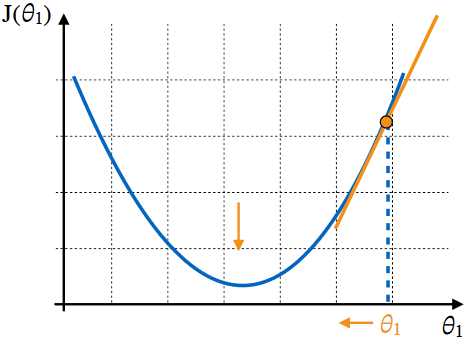
\includegraphics[width=0.4\textwidth]{images/GradientDescent1.png} & &
    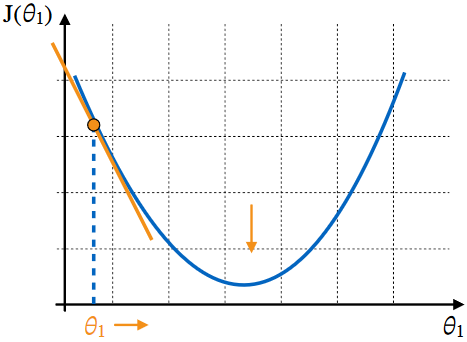
\includegraphics[width=0.4\textwidth]{images/GradientDescent2.png} \\
    \\
    $\eta$ too small & &
    $\eta$ too big \\
    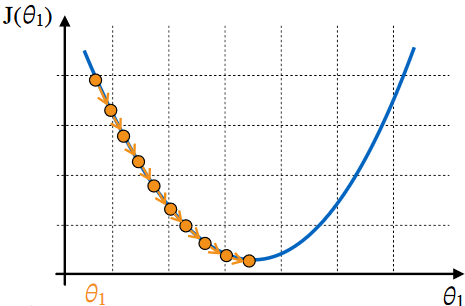
\includegraphics[width=0.4\textwidth]{images/GradientDescent3.png} & &
    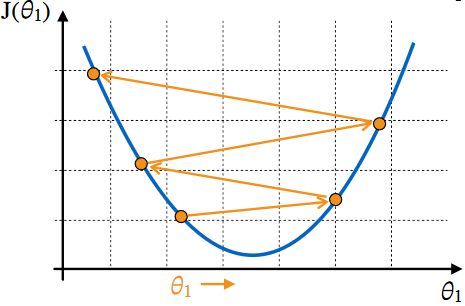
\includegraphics[width=0.4\textwidth]{images/GradientDescent4.png}
    \end{tabular} 
\end{center}

\newpage